\documentclass[a4paper,11pt]{article}
\usepackage{f420}

\captionsetup{width=0.8\textwidth}

\begin{document}

\section{\bf Range-деревья}

\emph{Range-дерево (дерево параллелепипедов)}~— структура данных, позволяющая
хранить \(n\)~то\-чек \(p_1, p_2, \ldots, p_n \in \br^d\) и отвечать на
запросы вида «сколько точек \(p_i\) находится в параллелепипеде
\([x^1_1, x^1_2] \times \ldots \times [x^d_1, x^d_2]\)»
за время \(O (\log^{d-1} n)\); при этом построение структуры данных
для \(n\) точек занимает время \(O (n \cdot \log^{d-1} n)\).


\begin{figure}[h] \centering
  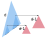
\includegraphics{img/range-tree}
  \caption{Ассоциированные структуры: в каждом внутреннем узле
    \(d\)-мерного дерева параллелепипедов~— \(d-1\)-мерное
    дерево, построенное для множества всех точек \(p_i\) под данным узлом}
  \label{fig:range-tree}
\end{figure}


\begin{theorem}
  Пусть \(d > 2\); запрос к \(d\)-мерному дереву сводится к
  \(\log n\) запросам к \(d-1\)-мерным деревьям.
\end{theorem}

Вспомним, как устроен запрос к одномерному дереву отрезков~— будем
рекурсивно спускаться из корня, и в текущей вершине для каждого из двух детей:
\begin{itemize}
  \item если отрезок, накрываемый им, не пересекает диапазон
    из запроса, — не вызываемся от этого ребёнка,
  \item если отрезок, накрываемый им, полностью содержится в диапазоне
    из запроса, — прибавляем к ответу количество точек, находящихся
    в листьях под этим ребёнком (это количество хранится
    непосредственно в нём);
  \item если отрезок, накрываемый им, пересекается с диапазоном
    из запроса, — вызываемся от него рекурсивно.
\end{itemize}

В общем, дерево отрезков в точности накрывает диапазон из запроса
поддеревьями \(\log n\) своих узлов, и ответ на запрос~— сумма
хранящихся в этих узлах количеств точек в листьях их поддерева.

\end{document}
